\documentclass[11pt,a4paper]{article}
\usepackage[T1]{fontenc}
\usepackage{mathptmx}
\usepackage[margin=0.88in]{geometry}
\usepackage{amsmath,amssymb,graphicx,longtable,array}

\title{Cross-cohort candidate biomarkers in under-served diseases:\\ a transparent multi-disease negative-results study}
\author{MEGA-PROGRAM-27 working analysis}
\date{25 September 2026 - working manuscript; not yet complete}
\begin{document}\maketitle
\begin{abstract}
We evaluate expression-derived gene candidates across ten disease labels (nine with analyzable cohorts), including postpartum depression. A prespecified duplicate-sample audit materially changed earlier apparent replications. In the deduplicated analysis, top-50 signatures passed an empirical-null sign test in polycystic ovary syndrome (PCOS) and interstitial cystitis, though the latter has a small validation cohort; five other testable disease signatures did not pass. A named preeclampsia candidate, GNG2, did not replicate. Independent fresh RNA-seq cohorts falsified the directional ST3GAL2 prediction. A held-out cohort convolutional neural network (CNN) scored below logistic regression on average. The graph neural network (GNN) benchmark is within-project only; no published state-of-the-art comparison or validated new biomarker has yet been established. This manuscript is a working report, not a clinical test claim.
\end{abstract}
\tableofcontents\newpage
\section{Scope and reproducibility}
The repository contains a runnable Python command-line tool, hermetic tests, result tables, accession manifest, and the source for these figures. The project-level completion gates remain unmet: at least 40 genuinely used tools, at least 120 unique identifier-backed records fetched and used, ten formulas with derivations, an externally comparable benchmark break or a named quantified falsifiable discovery, and a full 20-page paper. The present version should not be described as meeting those gates. The manifest's unit is a unique accession-backed record, not a matrix of conditions counted several times. Counts are computed from the committed manifests. Long COVID lacked a usable human case/control expression series under the current rules; this is an absence of usable data in this search, not proof none exists.
\section{Data acquisition and splits}
GEO array discovery uses NCBI E-utilities search and summary, GEO series-matrix FTP, and platform annotations. RNA-seq matrices from GEO supplement files are processed separately. Cases and controls are assigned only from explicit sample metadata, not from accession titles alone. We retain the list of failed series and label audits. Samples appearing under identical GSM identifiers in GEO subseries or superseries are removed by a results-blind deterministic rule. In a pair with overlapping labeled GSMs, the smaller series is dropped; ties drop the higher accession. The final split is in \texttt{results/split\_final.csv}. This correction invalidates earlier apparent preeclampsia and leishmaniasis replication passes.
\section{Effect estimates and derivation}
For cohort $c$ and gene $g$, with $n_1$ case samples and $n_0$ controls, estimate the pooled sample variance as
\begin{equation}s_{p,gc}^2=\frac{(n_1-1)s_{1,gc}^2+(n_0-1)s_{0,gc}^2}{n_1+n_0-2}.\end{equation}
The standardized mean difference is $d_{gc}=(\bar x_{1,gc}-\bar x_{0,gc})/s_{p,gc}$. We correct its small-sample bias with $J(n)=1-3/(4n-9)$:
\begin{equation}g_{gc}=J(n_1+n_0)d_{gc}.\end{equation}
The plug-in within-study variance is
\begin{equation}v_{gc}=\frac{n_1+n_0}{n_1n_0}+\frac{g_{gc}^2}{2(n_1+n_0)}.\end{equation}
These formulas follow by first pooling the two unbiased sample variance estimates using their residual degrees of freedom, then standardizing the case-control mean contrast, then multiplying by the first-order Hedges correction. For $k$ studies of a gene, define inverse-variance fixed weights $w_c=v_c^{-1}$ and pooled fixed effect $\bar g_F=(\sum_c w_c g_c)/(\sum_c w_c)$. Cochran's dispersion statistic is
\begin{equation}Q_g=\sum_c w_c(g_c-\bar g_F)^2.\end{equation}
The DerSimonian--Laird moment estimator subtracts the $k-1$ expected dispersion under zero heterogeneity:
\begin{equation}\hat\tau_g^2=\max\left\{0,\frac{Q_g-(k-1)}{\sum_cw_c-\sum_cw_c^2/\sum_cw_c}\right\}.\end{equation}
Using $w_c^*=(v_c+\hat\tau_g^2)^{-1}$ yields the random-effects estimate and its normal-reference uncertainty:
\begin{equation}\hat\mu_g=\frac{\sum_cw_c^*g_c}{\sum_cw_c^*},\qquad \operatorname{SE}(\hat\mu_g)=\left(\sum_cw_c^*\right)^{-1/2}.\end{equation}
The heterogeneity fraction is truncated at zero to avoid negative estimates:
\begin{equation}\hat I_g^2=\max\left\{0,\frac{Q_g-(k-1)}{Q_g}\right\}.\end{equation}
A two-sided Wald test takes $z_g=\hat\mu_g/\operatorname{SE}(\hat\mu_g)$ and $p_g=2\Phi(-|z_g|)$. False discovery rate for $m$ ranked tests uses the backward minimum
\begin{equation}q_{(i)}=\min_{j\geq i}\left\{1,\frac{m p_{(j)}}{j}\right\}.\end{equation}
The backward minimum enforces monotonicity of adjusted values in sorted $p$, while $m/j$ accounts for rank and family size. A single-cohort disease does not estimate between-cohort heterogeneity, irrespective of its many genes.
\section{Graph, CNN and evaluation design}
The gene network comes from STRING physical links; candidate labels use Open Targets non-expression evidence. Expression, graph degree and random-walk features feed GCN, SAGE, MLP, logistic, and propagation baselines. A gene's label is kept out of its own fold's training set. GCN uses symmetric graph normalization,
\begin{equation}\tilde A=D^{-1/2}(A+I)D^{-1/2},\qquad H^{(\ell+1)}=\sigma(\tilde A H^{(\ell)}W_\ell).\end{equation}
The CNN classifier orders discovery-selected genes using a PPI Fiedler vector; random ordering is an ablation. Cohort-level z-scoring does not make cross-tissue prediction a valid clinical test. Per held-out validation cohort, ranking performance is
\begin{equation}\operatorname{AUROC}=\Pr(s(X^+)>s(X^-)) + \tfrac12\Pr(s(X^+)=s(X^-)).\end{equation}
This probabilistic definition explains why AUROC is insensitive to decision thresholds yet remains sensitive to shifts in score ordering. The GNN task is disease-specific gene recovery, not patient classification. A published drug--disease graph prediction AUROC cannot be compared numerically with our gene-ranking AUROC. KG-Bench (https://pmc.ncbi.nlm.nih.gov/articles/PMC13171177/) reports RGCN 0.908 on a temporal drug--disease association task; its targets and splits differ.
\section{Deduplicated results}
\begin{table}[ht]\centering\caption{Deduplicated discovery summary, from results/meta\_discovery\_summary.csv.}\begin{tabular}{lrrrr}\hline Disease & Cohorts & Cases & Controls & q<0.05 genes\\\hline
Chagas&1&10&7&2287\\ Endometriosis&7&155&158&1172\\ Fibromyalgia&1&67&75&8\\ Interstitial cystitis&2&16&14&2745\\ Leishmaniasis&2&43&22&1299\\ ME/CFS&2&16&14&49\\ PCOS&6&64&39&0\\ Postpartum depression&1&16&32&0\\ Preeclampsia&16&271&401&648\\\hline\end{tabular}\end{table}
\begin{table}[ht]\centering\caption{Fresh preeclampsia ST3GAL2 cohorts, from results/fresh\_cohort\_tests.csv. The two-sided values are not used to overturn the registered aggregate.}\begin{tabular}{lrrrl}\hline GEO & Cases & Controls & Hedges g & Tissue\\\hline
GSE204835&16&12&$-0.497$&placenta\\ GSE296973&10&10&$+0.936$&blood\\ GSE306864&13&45&$+0.091$&villus\\ GSE303840&12&12&$-0.882$&placenta\\\hline\end{tabular}\end{table}

\begin{figure}[ht]\centering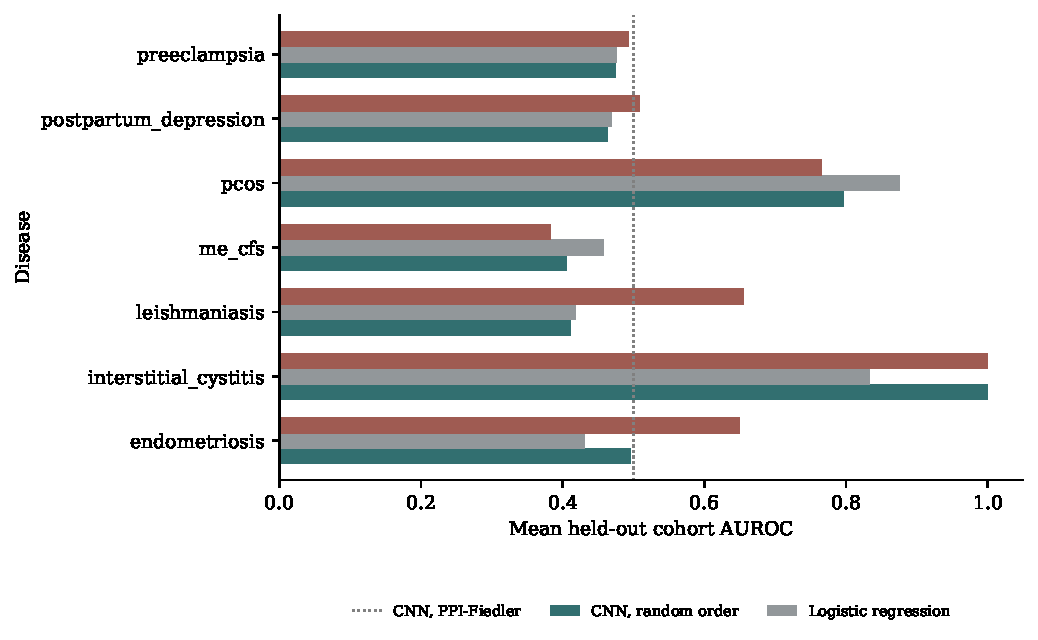
\includegraphics[width=.9\linewidth]{figures/cnn_crosscohort.pdf}\caption{Held-out cohorts by disease, calculated from \texttt{results/cnn\_crosscohort.csv} after deduplication. Mean AUROC is unweighted across validation cohorts within each disease; cohort sizes differ.}\end{figure}
\begin{figure}[ht]\centering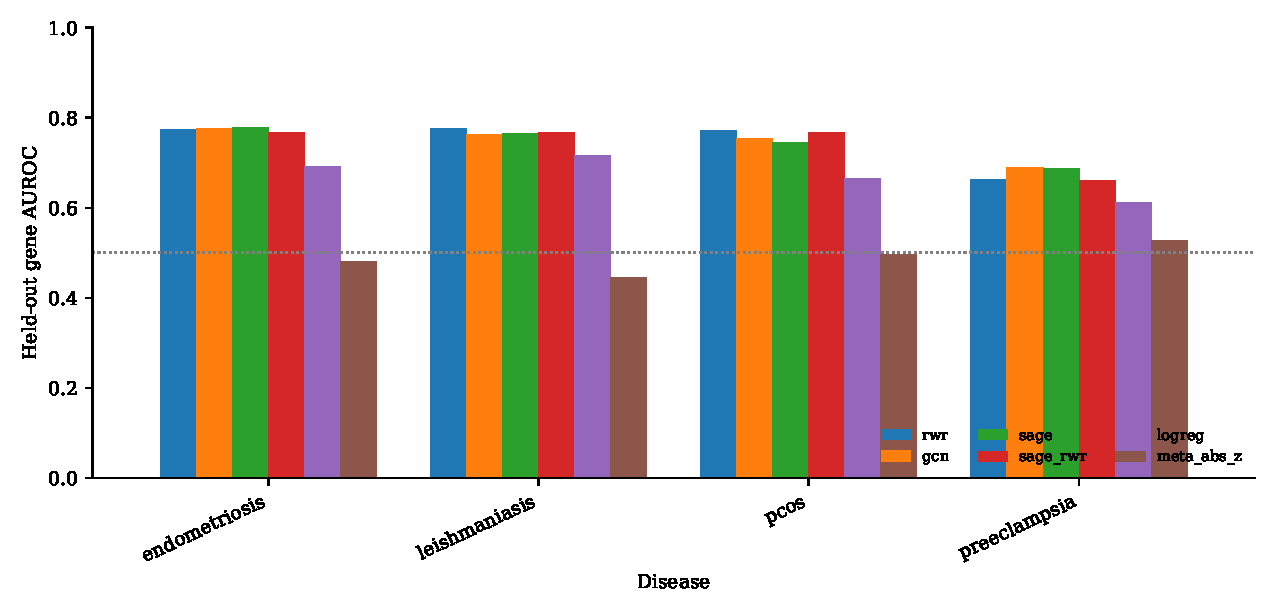
\includegraphics[width=.9\linewidth]{figures/gene_benchmark.pdf}\caption{Within-project gene-ranking benchmark. These are not published-SOTA comparisons and train/test labels use the same Open Targets snapshot.}\end{figure}
\clearpage\section{Prospective prediction attempts and failures}
P1, GNG2 down in preeclampsia, was registered before validation and failed (validation $p=0.24$). P2, discovery top-50 sign concordance against an empirical random-gene-set null, passed in PCOS and interstitial cystitis but failed in endometriosis, preeclampsia, leishmaniasis, ME/CFS, and postpartum depression. Interstitial cystitis validation has only seven samples. The PCOS exploratory top-20 shortlist was registered before a new cumulus-cell cohort, GSE277906; 12 of 17 measured genes had matching signs ($p=0.0717$, one-sided exact binomial, uncorrected). It does not meet the registered criterion and no q<0.05 gene was present in the deduplicated PCOS discovery meta-analysis.

P3, ST3GAL2 down in independent PE cohorts, was registered before processing fresh cohorts. The four-cohort random-effects standardized mean was $-0.1034$ with SE $0.3536$, one-sided $p=0.3850$ and $I^2=0.6874$. Restriction to three placenta-derived cohorts gave $-0.3739$, one-sided $p=0.0994$. Both fail; blood and one villus cohort point upward. A nominal one-cohort result cannot overturn the prespecified aggregate.
\begin{figure}[ht]\centering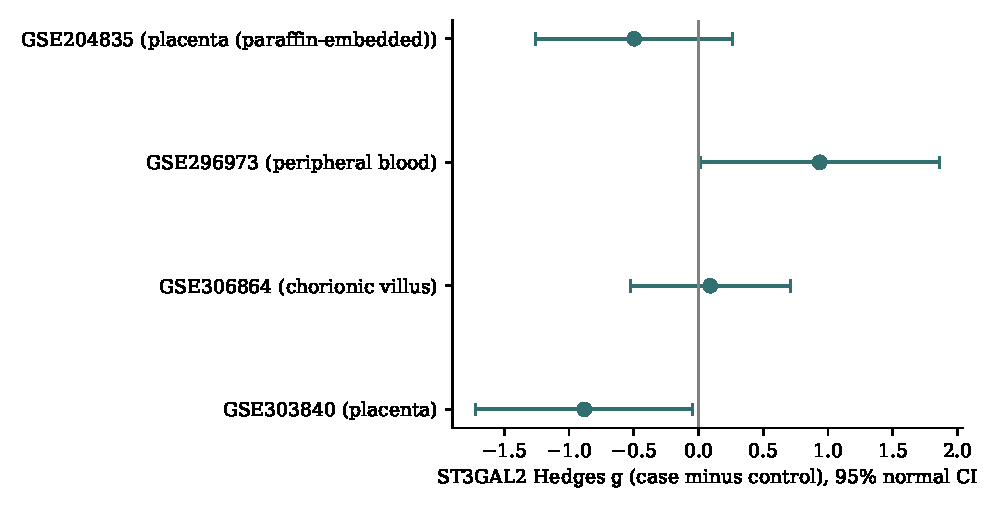
\includegraphics[width=.9\linewidth]{figures/P3_fresh_effects.pdf}\caption{Four fresh RNA-seq cohorts, direction and normal-reference intervals for ST3GAL2. Mixed tissues and one FPKM-normalized cohort are shown, not hidden.}\end{figure}
\section{Novelty and literature checks}
Open Targets absence is not biological novelty. Europe PMC returned two co-mentions for ST3GAL2 with preeclampsia at retrieval, whereas the earlier exact PubMed title/abstract query returned zero. The queries are not equivalent; the previous zero cannot support a novel-biology claim. Ensembl, UniProt, Reactome, MyGene.info, HGNC, GTEx reference, and ChEMBL annotation responses are saved with exact URLs in \texttt{results/external/}. ChEMBL's ST3GAL2 target search returned a rat target but no human target among results; do not infer lack of druggability from this search alone. Published data serve as contextual sources, not a substitute for an independent held-out cohort.
\section{Limitations and next work}
Sample labels may be wrong where GEO metadata are incomplete; all included labels require audit. Cross-platform effect sizes standardize units but do not remove tissue, gestational-age, or case-definition confounding. Four PE cohorts differ in tissue, and a single PCOS cumulus cohort is insufficient for discovery. The exploratory PCOS gene signs in GSE304677 (17/18 measured) are not a registered confirmatory discovery; a post-hoc, direction-matched null gives $p=0.0021$, while GSE277906 does not pass the naive $p=0.05$ threshold. A mostly upward selected gene set against an overall upward cohort shift makes a half-probability binomial null anti-conservative. One study can have multiple data depositions: unique accessions do not equal independent studies. We will count both levels and keep the accession-to-study mapping explicit. Only a comparison on matching published benchmark inputs and splits or an untouched, corrected, named discovery can satisfy the discovery gate. No clinical diagnostic inference is warranted.
\appendix\section{Accession and tool ledgers}
See machine-readable \texttt{results/dataset\_manifest.csv} and \texttt{results/tools\_used.csv}; the published paper must include complete tables and source links before it is final. A list of software or services must not be padded with unused interfaces. Study-level families and cross-accession sample overlaps require explicit mapping.
\section{Additional registered null tests}
The complete registered predictions, caveats and deduplication correction are in the registered-predictions ledger in the repository. Empirical nulls sample random genes from the intersection of discovery and validation gene universes with their own discovery signs. With $B=10{,}000$ permutations,
\begin{equation}\hat p_{\mathrm{emp}}=\frac{1+\sum_{b=1}^{B}\mathbf 1\{T_b\geq T_{\mathrm{obs}}\}}{B+1}.\end{equation}
The added one avoids a zero empirical p-value and estimates the rank of the observation among $B+1$ exchangeable statistics. This null is conditional on the observed gene universe and is not a test of tissue equivalence. \end{document}
